\documentclass[8pt,a4paper,compress,handout]{beamer}

\usepackage{/home/siyer/lib/slides}

\title{What is Computer Science?}
\date{}

\begin{document}
\begin{frame}
\begin{flushright}
\tiny \textsc{Computer science is no more about computers than astronomy is about telescopes. \\ - Edsger Dijkstra}
\end{flushright}
\titlepage
\end{frame}

\begin{frame}
\frametitle{Outline}
\tableofcontents
\end{frame}

\section{What is Computer Science?}
\begin{frame}[fragile]
\emph{Computer science} is the study of automating processes that scale. 

\bigskip

A \emph{computer scientist} is someone who specializes in the theory of computation and the design of computational systems.

\bigskip

Important concepts at the heart of computer science are: 
\begin{itemize}
\item data;  
\item algorithms; 
\item programming; 
\item abstraction; and 
\item problem solving and creativity.
\end{itemize}
\end{frame}

\section{Data}
\begin{frame}[fragile]

We live in an era of data overload. For example:
\begin{itemize}
\item Google, when searched for ``Alan Turing'', finds approximately 9.7 million pages, ranked in order of estimated relevance and usefulness; 
\item Facebook has approximately 1 billion active users who generate over 3 billion comments and ``Likes'' each day; 
\item GenBank, a national database of DNA sequences used by biologists and medical researchers studying genetic diseases, has over 100 million genetic sequences with over 100 billion DNA base pairs; and 
\item the Large Hadron Collider (LHC) at CERN produces collision data at the rate of 25 petabytes ($1 \text{petabyte} = 10^{15}$ bytes) per year.
\end{itemize}

\bigskip

All these data would be junk without ideas and tools from computer science.
\end{frame}

\section{Algorithms}
\begin{frame}[fragile]
An \emph{algorithm} is a precise sequence of steps for carrying out a task, such as ranking web pages in Google, searching for a friend on Facebook, or finding closely related genes in GenBank.

\bigskip

Example: an algorithm to estimate $\pi$.

\bigskip

\begin{minipage}{200pt}
\begin{enumerate}
\item Draw a square that is 2 by 2 feet.
\item Inscribe a circle of radius 1 foot (diameter 2 feet) inside this square.
\item Grab a bucket of $n$ darts, move away from the dartboard, and put on a blindfold.
\item Take each dart one at a time and for each dart:
\begin{enumerate}[a.]
\item With your eyes still covered, throw the dart randomly (but assume that your throwing skills ensure that it will land somewhere on the square dartboard).
\item Record whether or not the dart landed inside the circle.
\end{enumerate}
\item When you have thrown all the darts, divide the number that landed inside the circle by the total number, $n$, of darts you threw and multiply by 4. This will give you your estimate for $\pi$.
\end{enumerate}
\end{minipage}\hfill %
\begin{minipage}{100pt}
\begin{center}
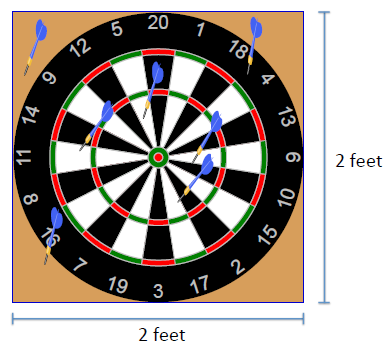
\includegraphics[scale=0.3]{figures/estimating_pi.png}

\smallskip

\tiny Estimating $\pi$
\end{center}
\end{minipage}
\end{frame}

\section{Programming}
\begin{frame}[fragile]
A \emph{program} is a list of instructions used to control the behavior of a computer, and a \emph{programming language} is a formal language designed to communicate those instructions to the computer.

\bigskip

\begin{minipage}{200pt}
Types of programming languages:
\begin{itemize}
\item machine languages -- interpreted directly in hardware; 
\item assembly languages -- thin wrappers over corresponding machine languages; 
\item high-level languages -- machine independent; 
\item system languages -- designed for writing low-level tasks, like memory and process management; 
\item scripting languages -- generally extremely high-level and powerful; 
\item domain-specific languages -- used in highly special-purpose areas only; 
\item visual languages -- non-text based; and
\item esoteric languages -- mostly of academic interest.
\end{itemize}
\end{minipage}\hfill %
\begin{minipage}{100pt}
\begin{center}
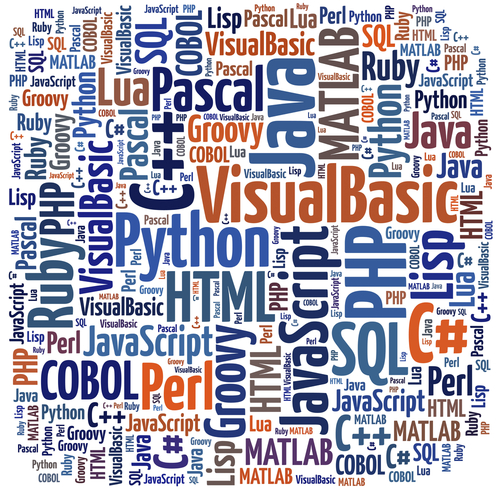
\includegraphics[scale=0.9]{figures/programming_languages.jpg}

\smallskip

\tiny Programming languages
\end{center}
\end{minipage}%

\bigskip

In this course we'll learn about the PicoBot (domain-specific), HMMM (assembly), and Python (scripting) programming languages.
\end{frame}

\section{Abstraction}
\begin{frame}[fragile]
\emph{Abstraction}, a key idea in the design of any large system, is the idea that when designing one part of a program, we can ignore the inessential details of other parts of the program as long as we have a high-level understanding of what they do.

\bigskip

In the design of software systems, abstraction ensures that many people can contribute to the project without everyone needing to understand everything, test the software methodically, and update it in the future by simply replacing an old component with a new and improved one. 
\end{frame}

\section{Problem Solving and Creativity}
\begin{frame}[fragile]
Computer science is an enormously creative endeavor that requires innovative problem-solving, exploration, and even experimentation.

\bigskip

Often times, there's more than one way to solve a problem and in some cases there's not even a clear ``best'' way to solve a problem.

\bigskip

While Google, Facebook, and GenBank are wonderfully easy to use, many challenges arose and continue to arise in the design and continual updating of such systems. 
\end{frame}

\end{document}
